\chap{Discussion and Extended Evaluations}

The current study investigates the possibility of testing the Data Science process using Python, trying to apply it to the Norwegian salmon farming industry, in order to gather and let be available as many useful results as possible.

\section{Evaluations of the study}
During this work is shown that is actually possible to have a first approach to the Data Science field using Python. All the documented steps of this works allow to have a complete overview of the general Data Science process.

Furthermore, the resulting Python systems and the corresponding evidences are showing which modules and packages are provided by Python in order to analyze, display and forecast data values. The high reusability and automation levels of the implemented system allow to easily reuse it in order to apply the same analysis, displaying and forecasting on a different dataset that contains data from a different area of interest. \\
On the other side the current system is probably efficient and productive for a personal use. That's because is not provided an implemented GUI, and to customize the system's outputs you have to have some basic knowledge of Python language, that could be a limitation for several people, but it could also be considered like an incentive for people to get to know this powerful programming language.

The approach used for this thesis didn't provide any kind of results that can be considered as new information about the Norwegian salmon farming field, but it provided a new way to visualize large amounts of data and also several discussion's starting points for further works. That's because this thesis was mainly focused on the Data Science process, Python utilities and to find out observations for future researches instead of the information extraction process itself.

Even that, as reported in the Results Overview chapter, several systems, evidences and values have been calculated and reported during this work. 

In the next sections are reported the discussions that I considered most relevant and interesting for further works, and then are reported the encountered limitations. 

\section{Considerations about implemented Evaluation System }
\label{Discussion1}
The following resulting table reveals several informations. \\
The column "Evaluation MAPE" is the average MAPE of the forecasted values during the Evaluation System with the reported ARIMA order. \\ 
The column "Forecast MAPE" represents the average MAPE of the 12 values predicted in the future, already reported in the results. [\ref{table: RealPredMAPE1}] 

 \begin{table}[ht]
\makebox[\textwidth][c]{
    \begin{tabular}{ | l | l | l | l | l |}
            \hline
\textbf{County} 	& \textbf{Parameter} & \textbf{ARIMA Order}	& \textbf{Evaluation MAPE} 	& \textbf{Forecast MAPE} 	\\ \hline
Finnmark 	& feedConsumption				& (6, 1, 0) 			& 13.771\% 	&	19.20\% 		\\ \hline	
Hordaland 	& feedConsumption				& (8, 0, 0)  			& 6.811\%	& 	17.89\%			\\ \hline				
Troms 		& feedConsumption				& (2, 0, 0)  			& 11.593\% 	&	43.04\%			\\ \hline
Nordland 	& feedConsumption				& (6, 0, 0)  			& 12.741\%	&	26.01\% 		\\ \hline
Norway0714 	& feedConsumption				& (6, 1, 0)  			& 7.296\%  	&	7.94\%			\\ \hline
    \end{tabular}}
         \caption{Comparison between Evaluation MAPE and Prediction MAPE}   
   \label{table: MAPE_Comparison} 
\end{table}        

From the values contained in the table [\ref{table: MAPE_Comparison}] is possible to see that the average MAPE for the forecasted future values (\textbf{Forecast MAPE}) is much higher than the one reported from the evaluation process (\textbf{Evaluation MAPE}) . \\
There is just one particular case where the Evaluation MAPE and Forecast MAPE values are really close, that is the one about the Norway dataset.

At this point, it would be extremely useful to discover why the predicted future values about the dataset 'Norway0714' are much more accurate and why their average MAPE is really close to the one calculated during the evaluation procedure.\\
In order to understand the reason, certain analysis through the resulting evidences have been made. Below here are reported the considerations about it:
\vspace{-5mm}
\begin{itemize}
 \item Checked the annual feed consumption trend during different years for the current datasets, that is possible to check out in the reported graphics [\ref{fig: Norway_feed}]. No big differences between the Norway's trend compared with the others was found.
 \item Checked correlation coefficients between different years of the feed consumption values for each tested dataset, but there were not any kind of significant high/low correlation levels with the years before.
 \item Tried to execute the prediction system with settings that are different by the one suggested in the Evaluation system results. Found that for some particular dataset is possible to get better predictions with a different configuration, like for example: \\
 Prediction system about "feed consumption" in Nordland executed with the suggested configuration (6,0,0) shows an average MAPE value equal to 26.01\% for the predicted values, like showed in the table [\ref{table: MAPE_Comparison}]. \\
If the Prediction system is tested on the same input but fitting the ARIMA model with the order (6,1,0) the average MAPE value decrease to 16.82\% for the predicted values. It's possible to clearly see this difference watching at the graphics reported in the following page: [\ref{fig: Nordland_ARIMAevaluation}] and [\ref{fig: Nordland_ARIMAmanual}]. \\ 
Furthermore, it's even possible to check in the table [\ref{table: MAPE_Comparison}] that the predictions about Troms, calculated with the suggested configuration (2, 0, 0),  gives a resulting Forecast MAPE of 43.03\%. But once tested with a manual configuration of (6, 1, 0) the resulting Forecast MAPE is decrease to 21.05\%.
\end{itemize}

This shows that the initial Evaluation system is not that accurate and reliable for each kind of input dataset. For this reason, in order to improve it during further works, is strongly suggest to try the "Box-Jenkinks method" for determine the best ARIMA order's parameters, that would probably be better and more specific for each single dataset. It provides a more accurate procedure for analyze a series, in order to determine the best ARIMA parameters to use. More details about it are reported in recommendation for further works.


\newpage

\begin{figure}[H]
	\makebox[\textwidth][c]{
    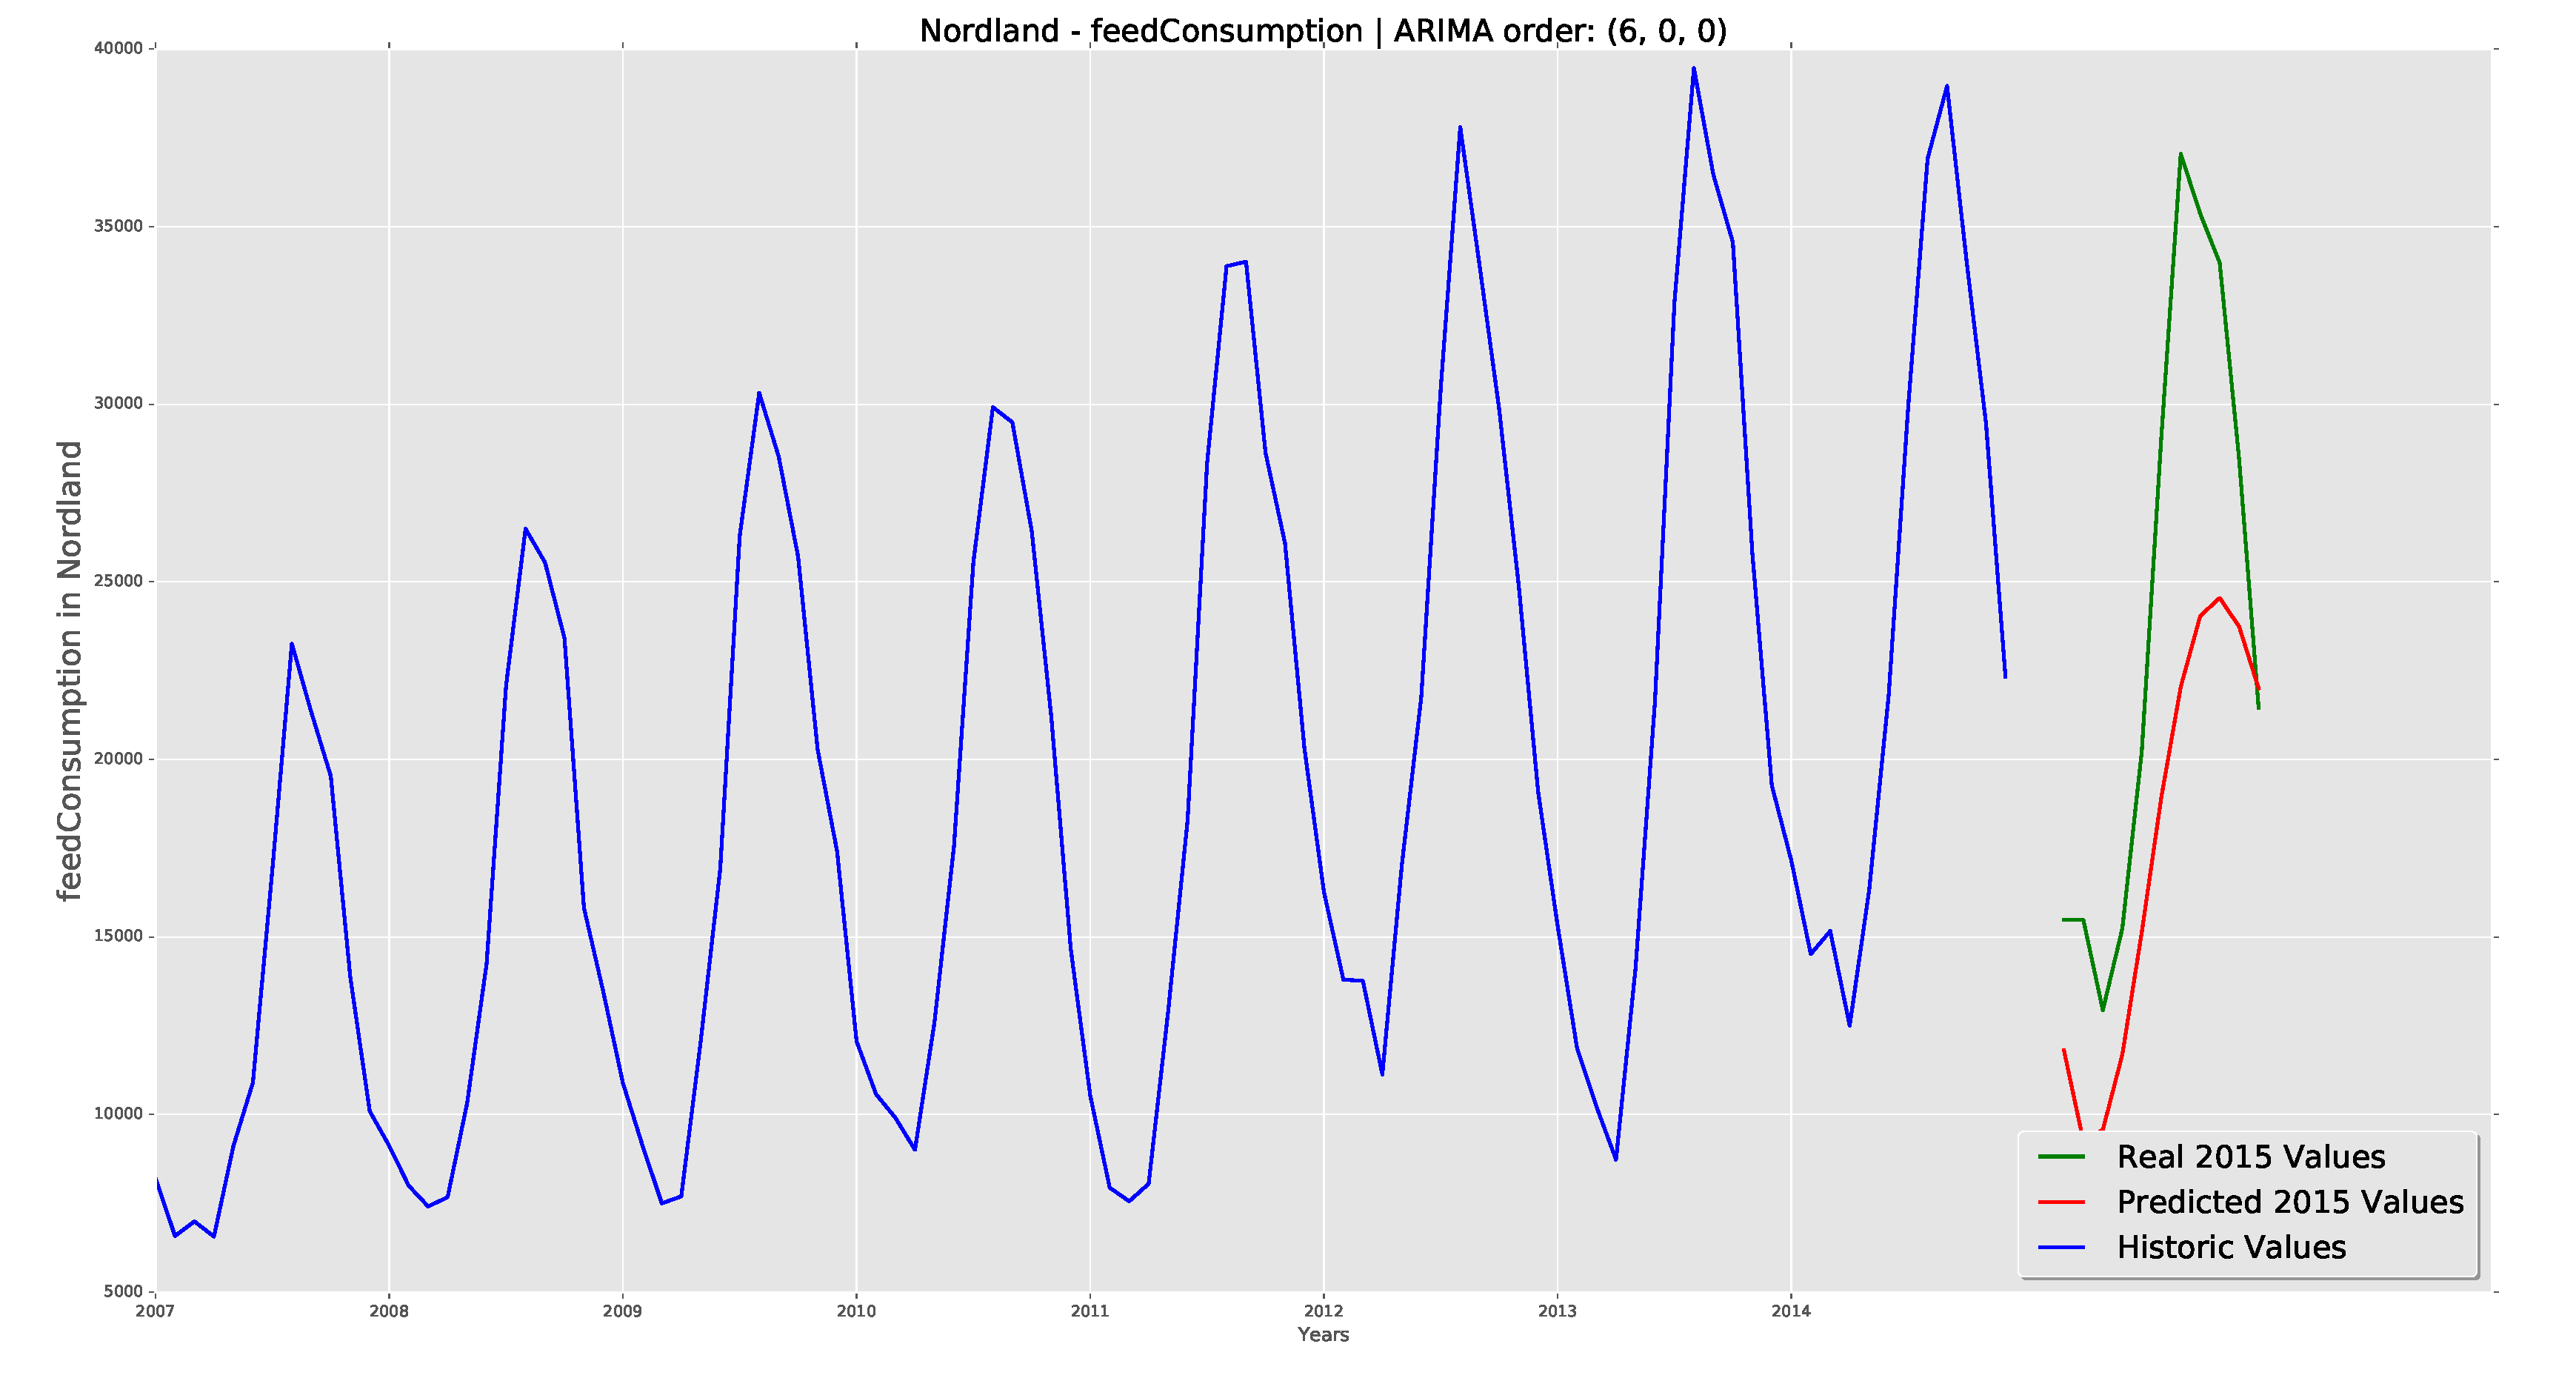
\includegraphics[trim={0 1cm 0 0},clip,width=1\textwidth]{Files/Nordland-feedConsumption_pred.pdf}}
    \caption[Predicted 2015 feed consumption in Nordland. Evaluation system ARIMA order.]{Predictions of 2015 feed consumption values in Nordland using ARIMA model fitted with the order suggested by the evaluation system results (6,0,0).\\  It provides an average MAPE of 26.01\% between the real and predicted 2015 values. }
    \label{fig: Nordland_ARIMAevaluation}
\end{figure}

\vspace{1cm}

\begin{figure}[H]
	\makebox[\textwidth][c]{
    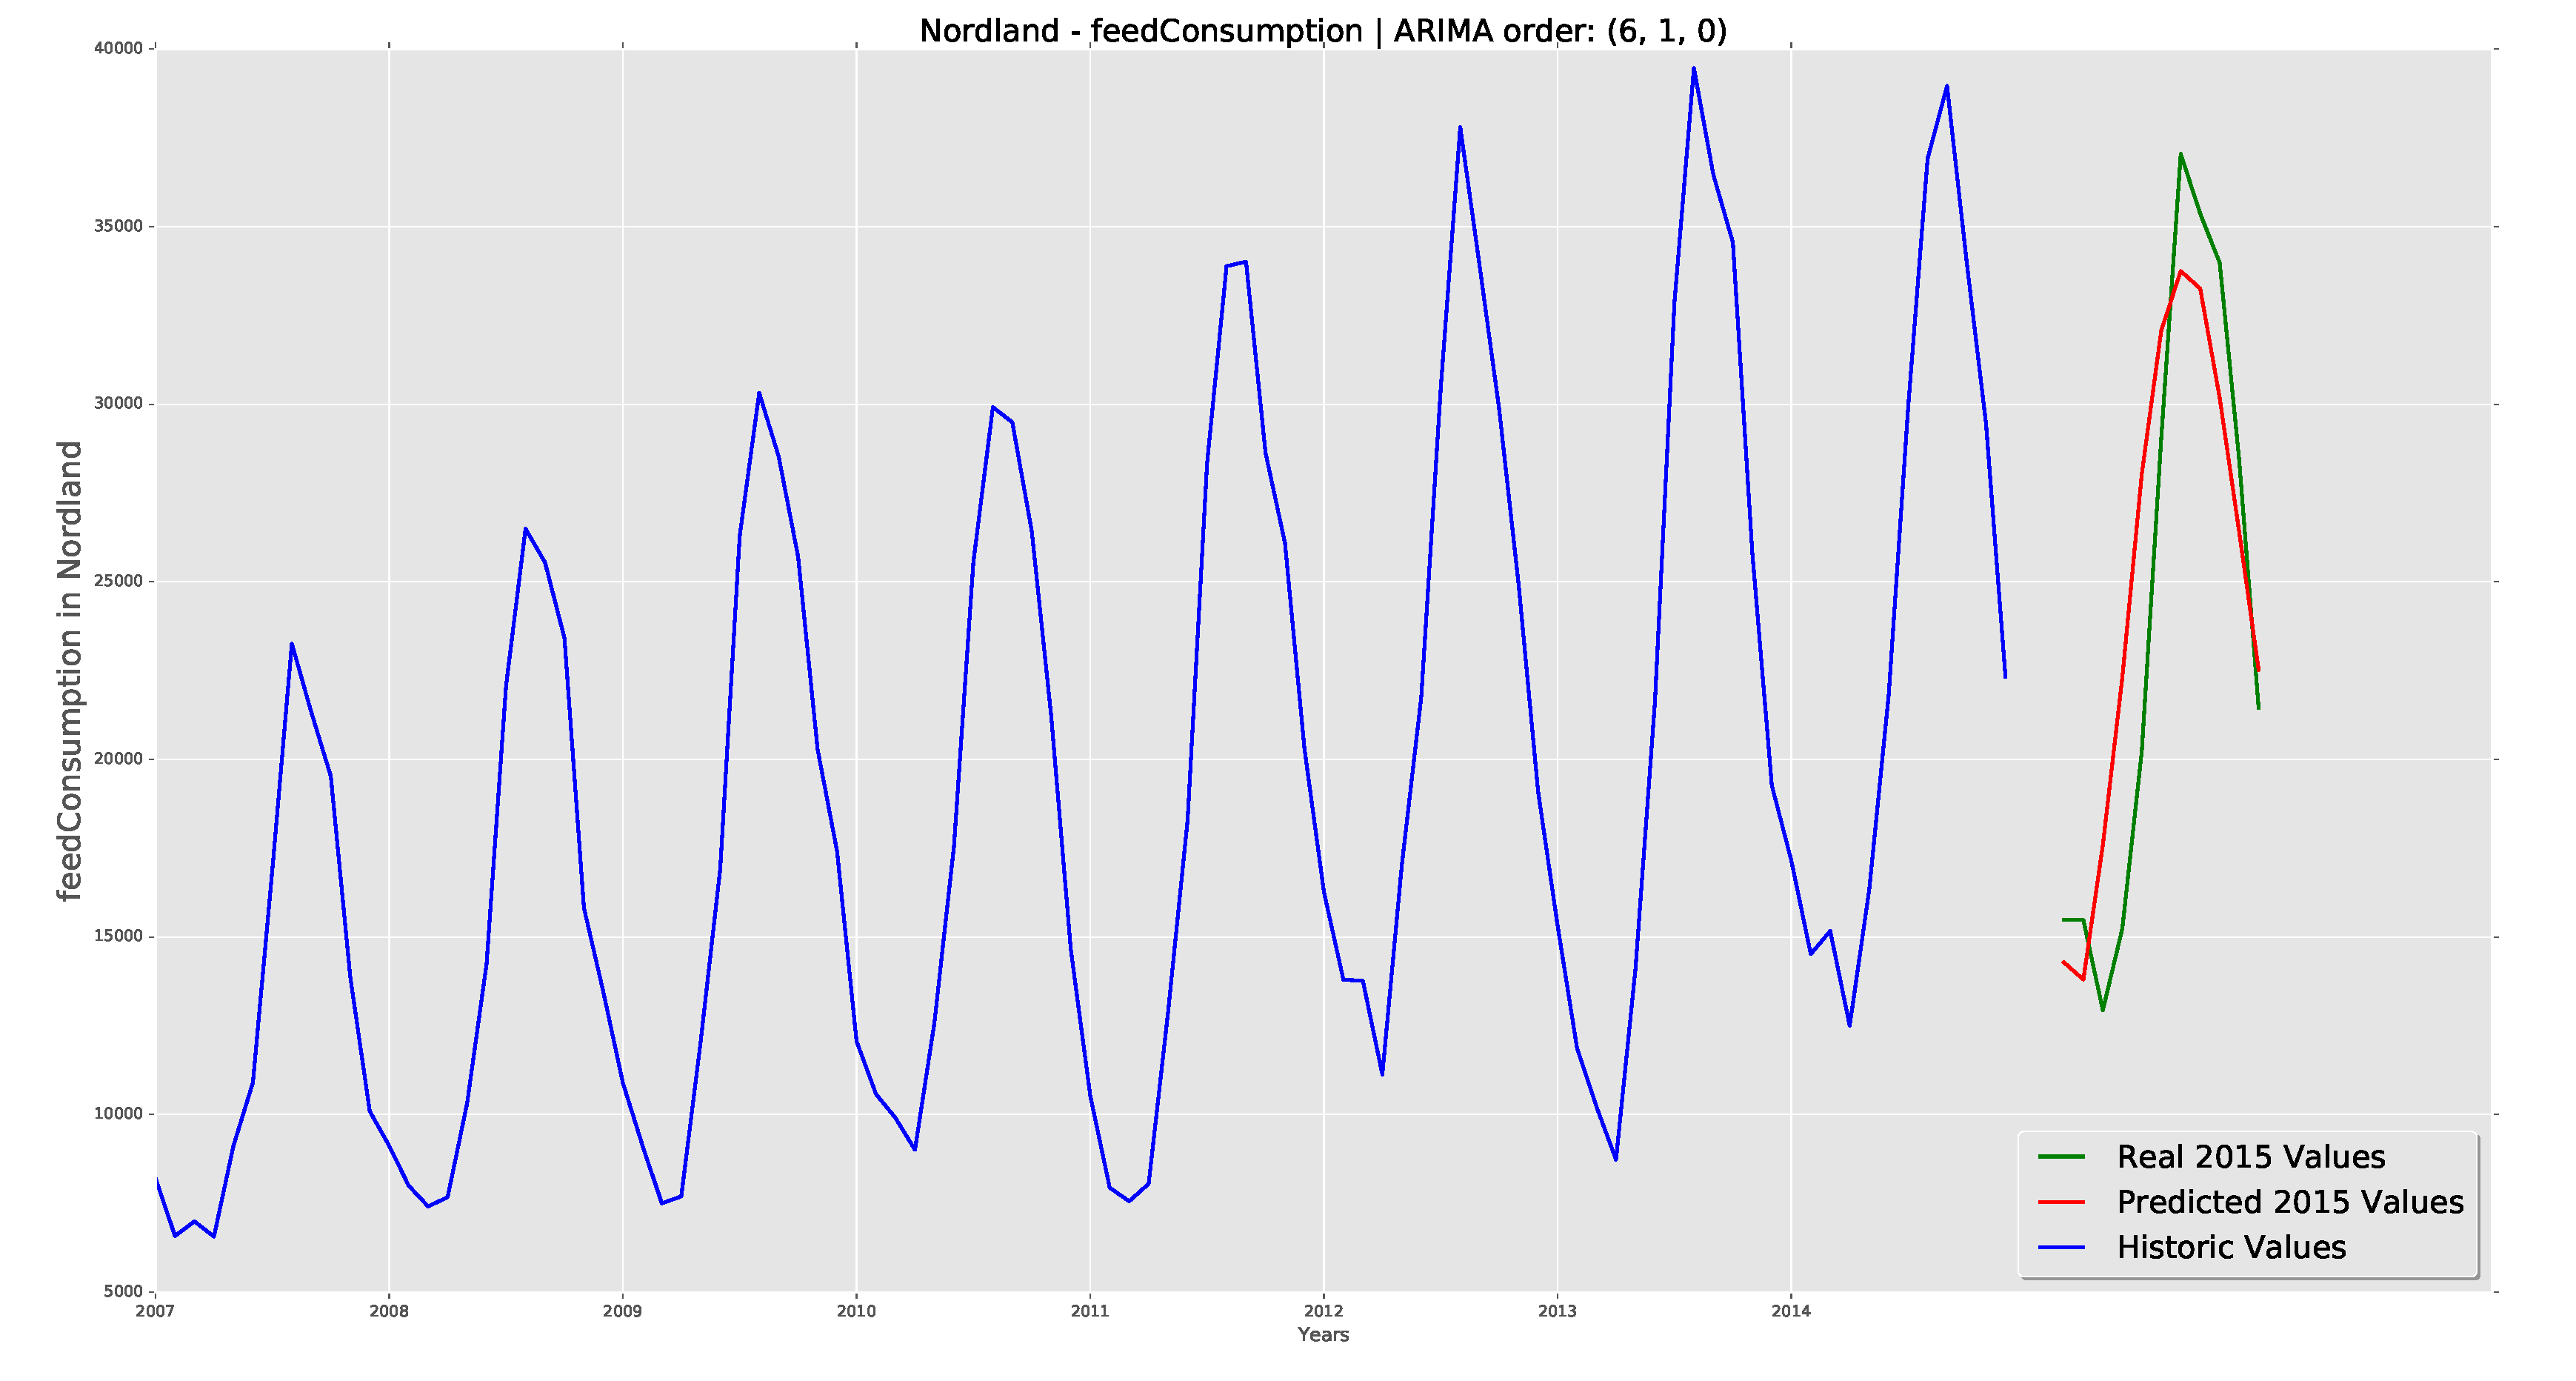
\includegraphics[trim={0 1cm 0 0},clip,width=1\textwidth]{Files/Nordland-feedConsumption_BETTER.pdf}}
    \caption[Predicted 2015 feed consumption in Nordland. Manual ARIMA order.]{Predictions of 2015 feed consumption values in Nordland using ARIMA model fitted with an order manually chosen (6,1,0).\\  It provides an average MAPE of 16.82\% between the real and predicted 2015 values. }
    \label{fig: Nordland_ARIMAmanual}
\end{figure}


\newpage

\section{Extended evaluations: feed consumption forecasting }
\label{Discussion2}
During the implementation of this work, was also noticed a strong relation between the two parameters "Sea Average Temperature" and "Feed Consumption".
I decided to focus on this particular correlation because, also if it's already well known that is possible to feed more the salmon when the temperature is higher, it could be very useful for further predictions about feed consumption values, since the sea average temperature would be considered like a parameter to use for improve the final results.

This correlation is significant for all the Norwegian counties and it's clearly possible to see it with the example graphic\footnote{The graphics reported above have been displayed with a Python system implemented during this study, that allows to display different parameters in a normalized range. The system has not been reported in the thesis work, but is possible to find it here named "Analysis.py": \\ \url{https://github.com/Sprea22/Personal_Utilities}} reported below here. 

\vspace{-10mm}

\makebox[1\textwidth][c]{
\begin{minipage}[t]{0.6\textwidth}
\begin{figure}[H]
    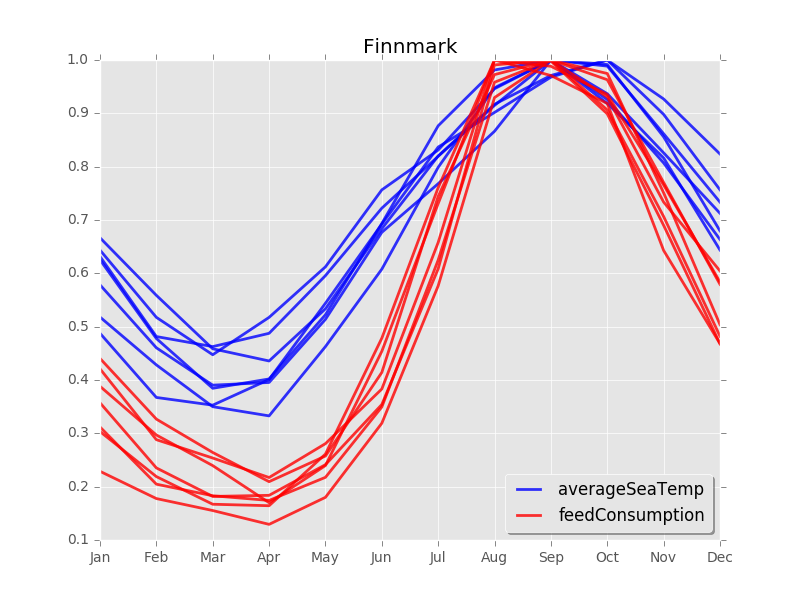
\includegraphics[trim={0 0.5cm 0 0},clip,width=1\textwidth]{Files/Finnmark-Temp&Feed.png}
    \caption[Finnmark: average sea temperature compared with feed consumption]{Comparison between average sea temperature and feed consumption in Finnmark}
    \label{fig: Finnmark_seaTemp&feed}
\end{figure}
\end{minipage} \hfill
\begin{minipage}[t]{0.6\textwidth}
\begin{figure}[H]
	\centering
    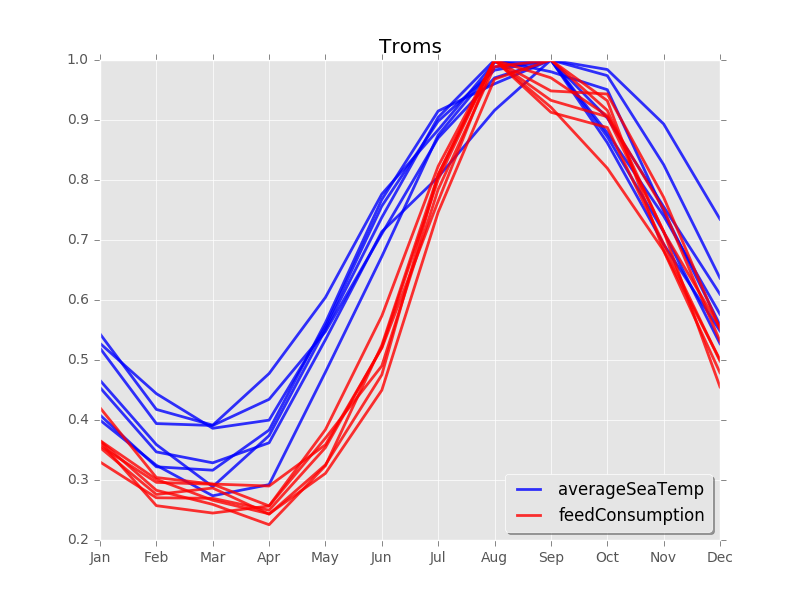
\includegraphics[trim={0 0.5cm 0 0},clip,width=1\textwidth]{Files/Troms-Temp&Feed.png}
    \caption[Troms: average sea temperature compared with feed consumption]{Comparison between average sea temperature and feed consumption in Troms}
    \label{fig: Troms_seaTemp&feed}
\end{figure}
\end{minipage}}
\makebox[1\textwidth][c]{
\begin{minipage}[t]{0.6\textwidth}
\begin{figure}[H]
    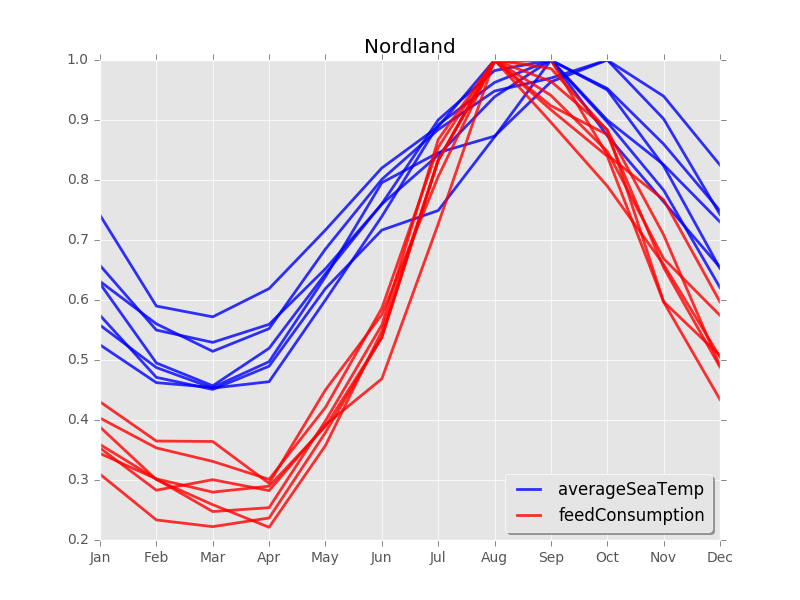
\includegraphics[trim={0 0.5cm 0 1cm},clip,width=1\textwidth]{Files/Nordland-Temp&Feed.png}
    \caption[Nordland: average sea temperature compared with feed consumption]{Comparison betwen average sea temperature and feed consumption in Nordland}
    \label{fig: Nordland_seaTemp&feed}
\end{figure}
\end{minipage} \hfill
\begin{minipage}[t]{0.6\textwidth}
\begin{figure}[H]
	\centering
    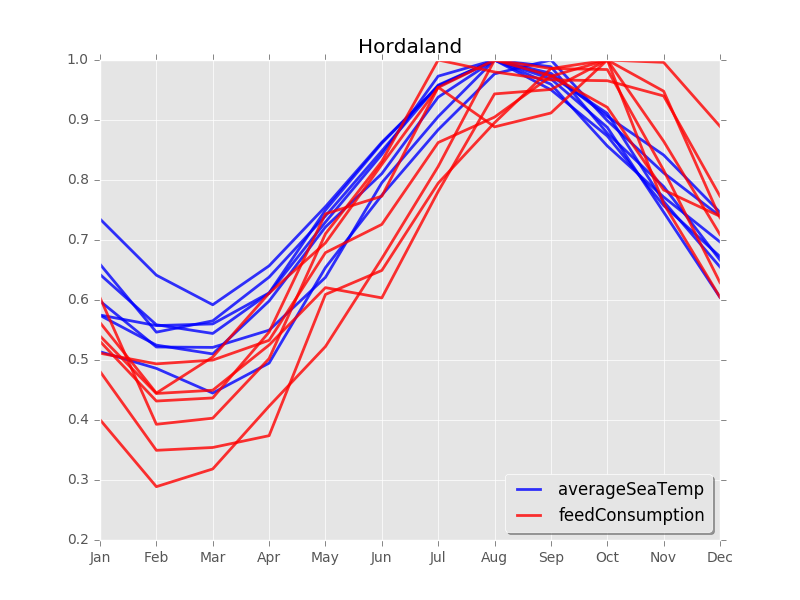
\includegraphics[trim={0 0.5cm 0 1cm},clip,width=1\textwidth]{Files/Hordaland-Temp&Feed.png}
    \caption[Hordaland: average sea temperature compared with feed consumption]{Comparison between average sea temperature and feed consumption in Hordaland}
    \label{fig: Hordaland_seaTemp&feed}
\end{figure}
\end{minipage}}

\newpage

The following graphics allow to have a very clear overview of what just written above.\\
\vspace{-10mm}
\begin{itemize}
 \setlength{\itemsep}{-5pt}
 \item In the first graphic the average sea temperature (Celsius) is reported , where blue means lower temperature and red higher temperature.
 \item In the second graphic the feed consumption per biomass (kg/kg) is reported , where red means an higher consumption and blue a lower one.
\end{itemize}

So it's clearly possible to see how the average sea temperature and the feed consumption per biomass have a significant correlation for every single Norwegian county.

\begin{figure}[H]
	\makebox[\textwidth][c]{
    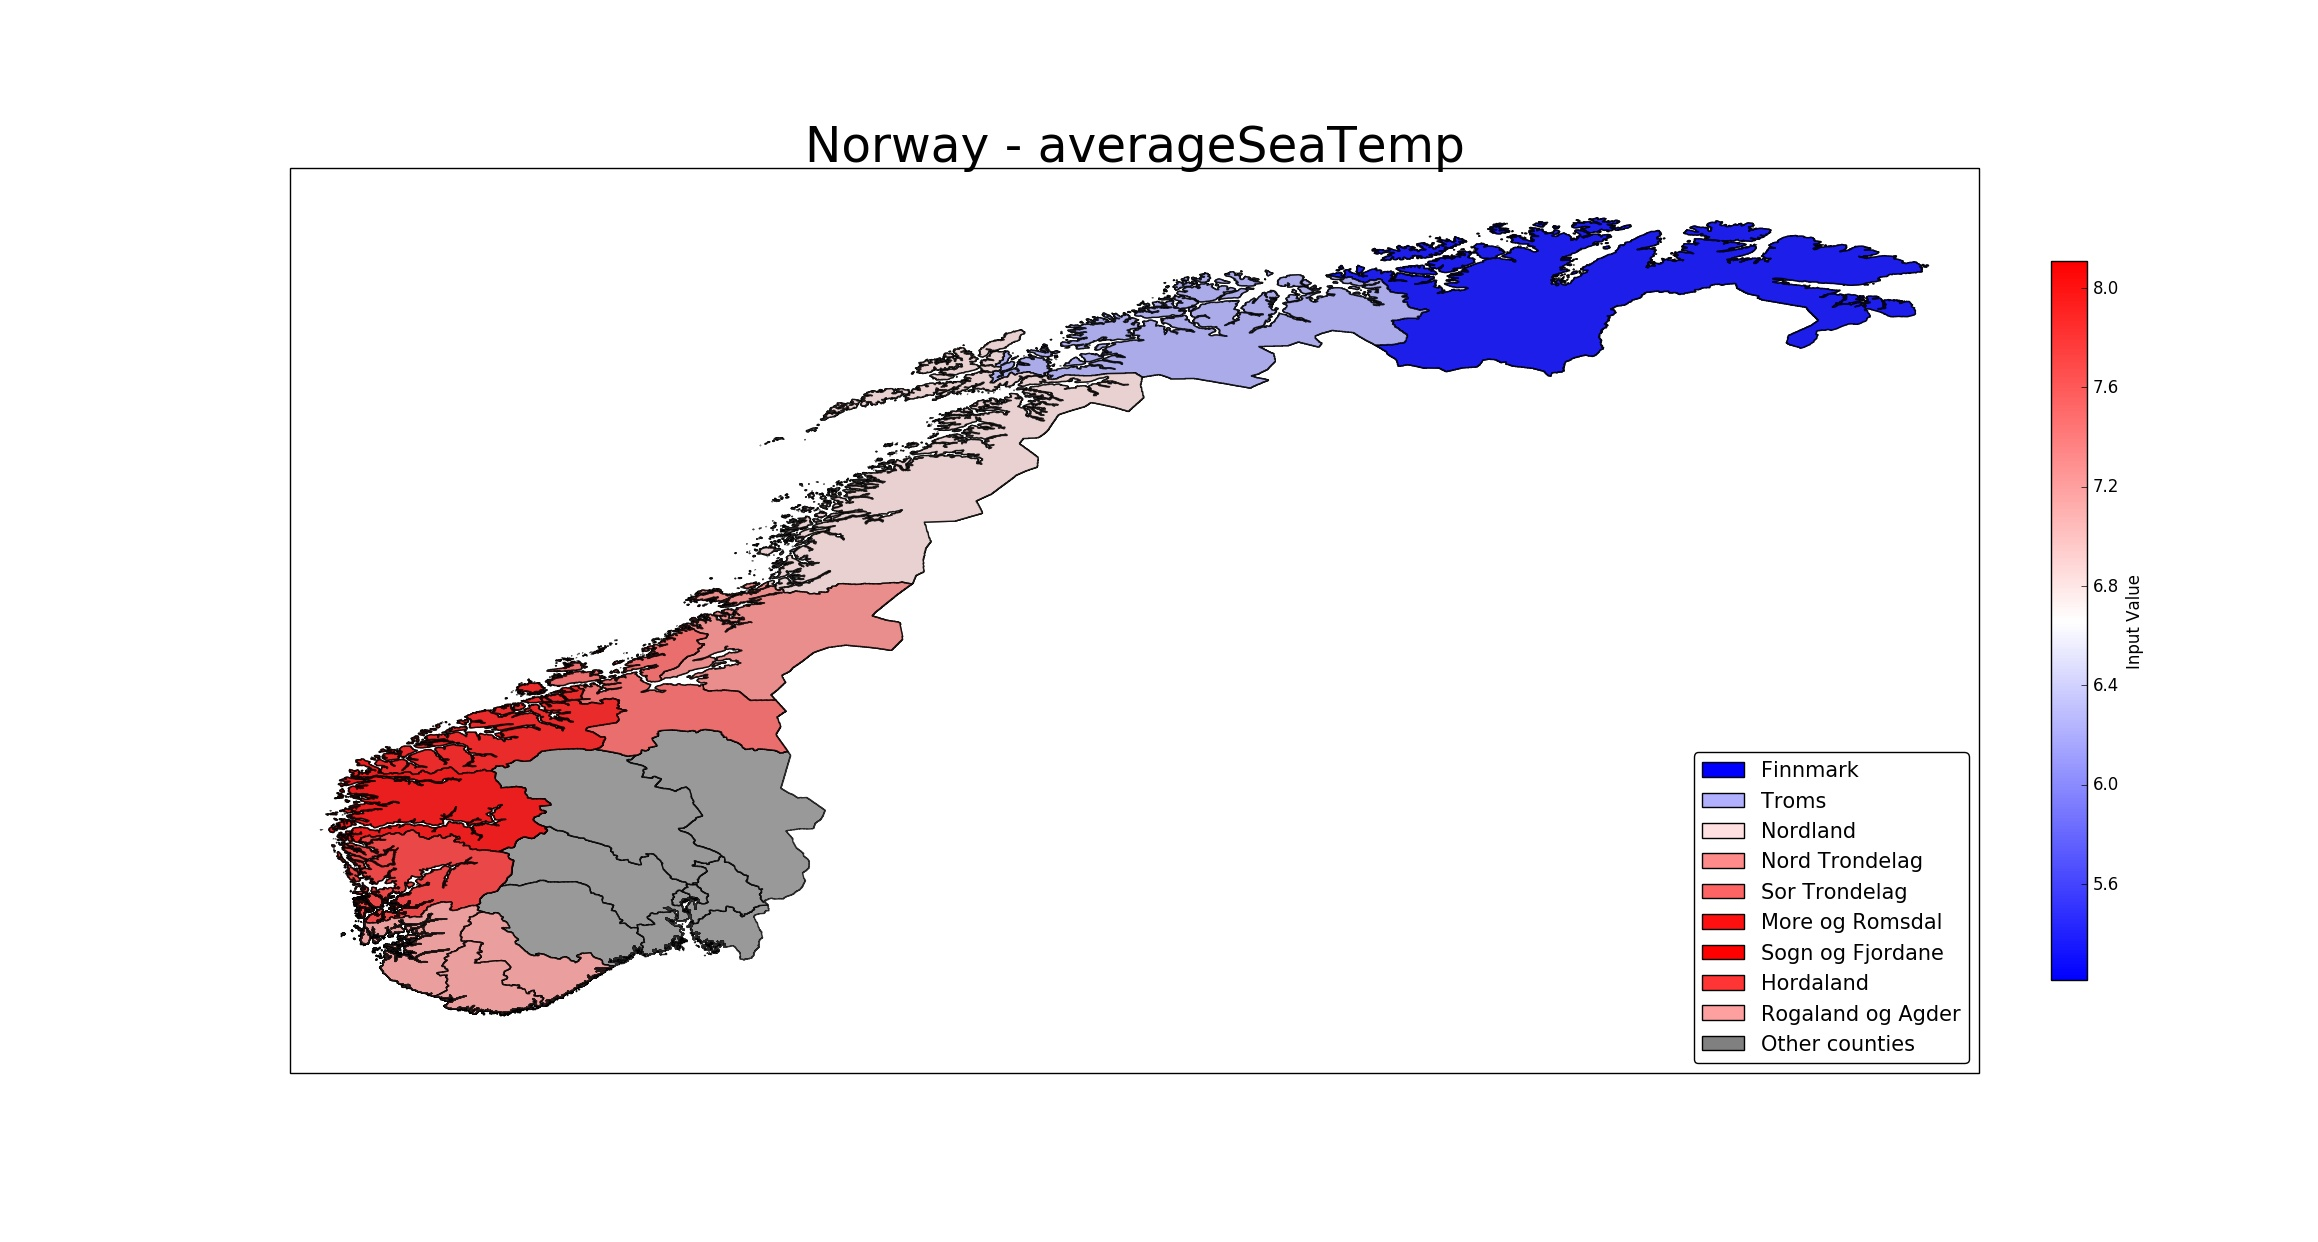
\includegraphics[trim={0 4cm 0 3cm},clip,width=1.3\textwidth]{Files/norway_averageSeaTemp.pdf}}
    \caption[Map: monthly average sea temperature in Norway]{Shows the average of the monthly average sea temperature (Celsius) from 2007 to 2014 in Norway}
    \label{fig: Norway_averageSeaTemp}
\end{figure}

\begin{figure}[H]
	\makebox[\textwidth][c]{
    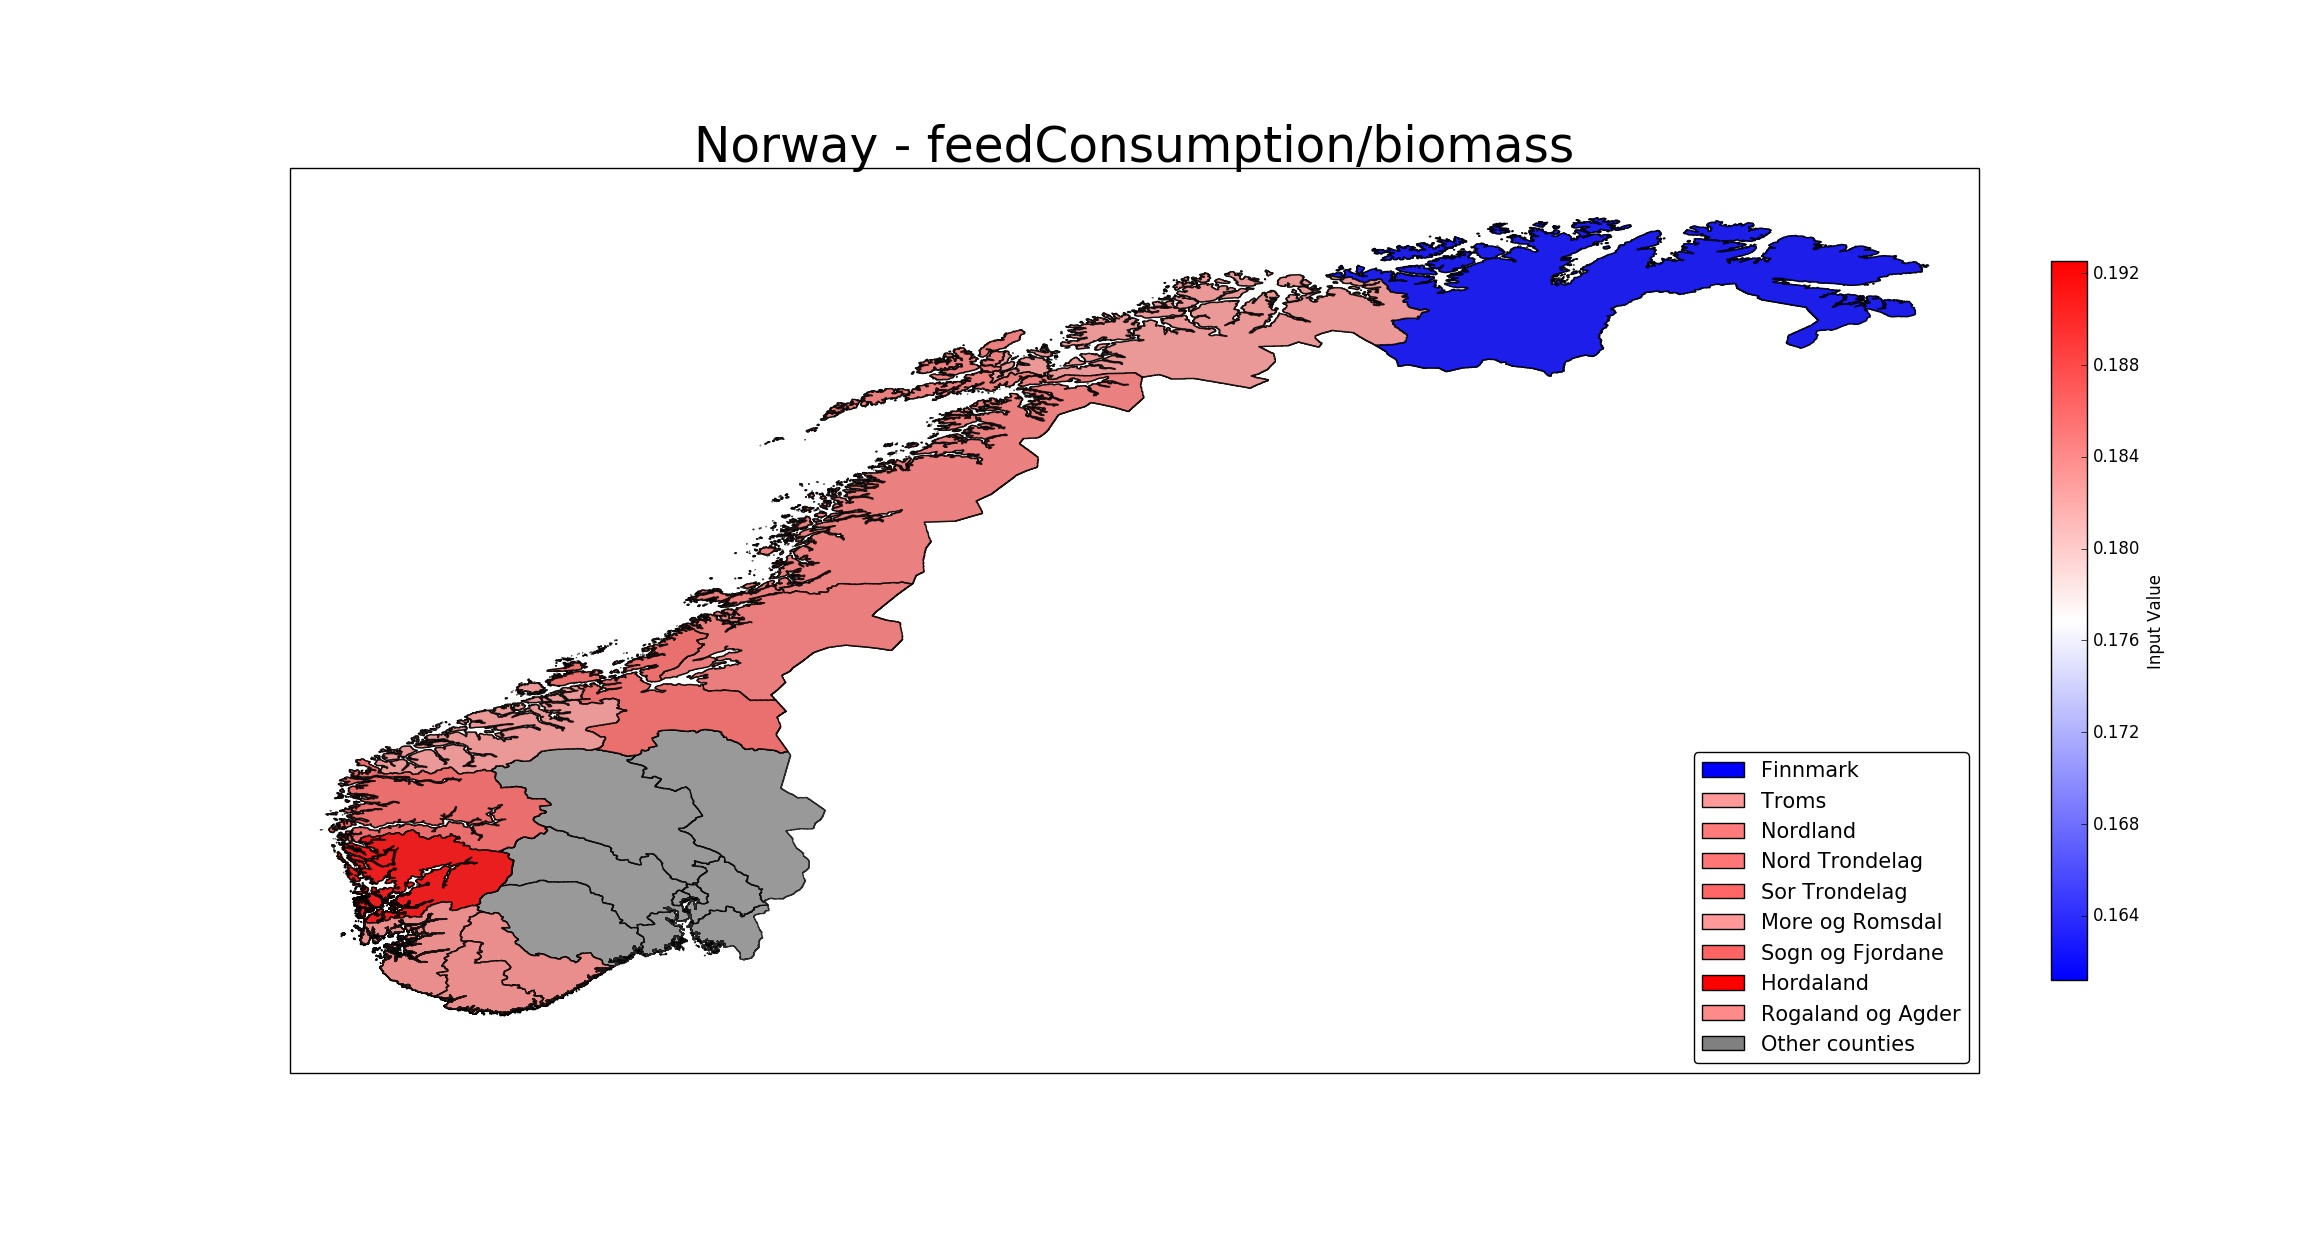
\includegraphics[trim={0 4cm 0 3cm},clip,width=1.3\textwidth]{Files/norway_feed-biomass.pdf}}
    \caption[Map: monthly average feed consumption / biomass in Norway]{Shows the average of the monthly average feed consumption per biomass (kg/kg)from 2007 to 2014 in Norway}
    \label{fig: Norway_feed-biomass}
\end{figure}

\newpage

Furthermore, it is even possible to check the correlation coefficient values reported in the correlation matrix below here. These graphic represent the correlation coefficient between different parameter about the same dataset (county in this case).\\
You can find the the correlation coefficient value's representation at the crossing point between "averageSeaTemp" and "FeedConsumption" of each correlation matrix represented below here.\\
It's possible to see that the correlation value's representation shows an high correlation value (red means high correlation) between the two parameters. Even if you check through the other Norwegian counties correlation matrix, this high correlation is valid.\\


  \vspace{-10mm}
  
\makebox[1\textwidth][c]{
\begin{minipage}[t]{0.6\textwidth}
\begin{figure}[H]
    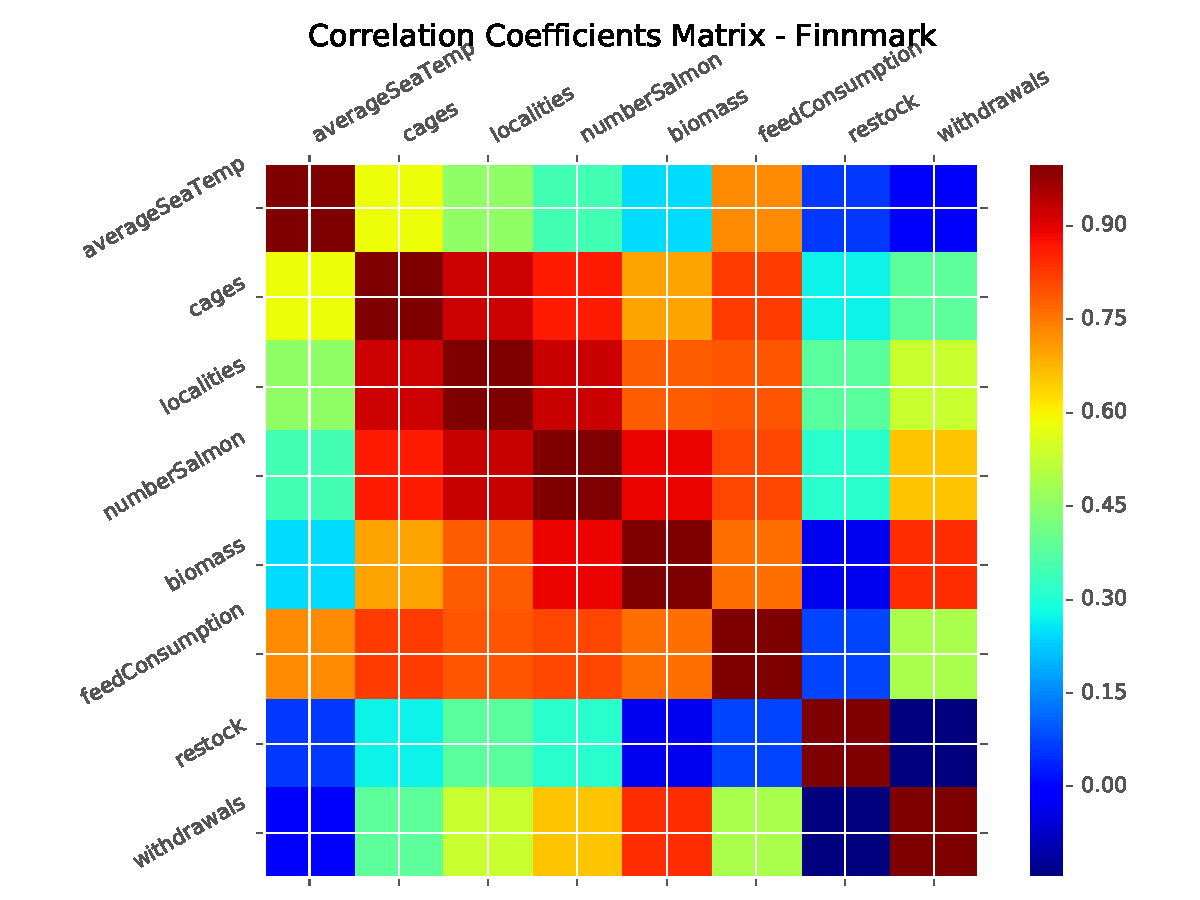
\includegraphics[trim={0 0 0 0},clip,width=1\textwidth]{Files/Finnmark_Total_Matrix.pdf}
    \caption[Correlation matrix between parameter of Finnmark dataset.]{Correlation matrix between all the parameters of the dataset about Finnmark}
    \label{fig: Finnmark_parametersComparison}
\end{figure}
\end{minipage} \hfill
\begin{minipage}[t]{0.6\textwidth}
\begin{figure}[H]
	\centering
    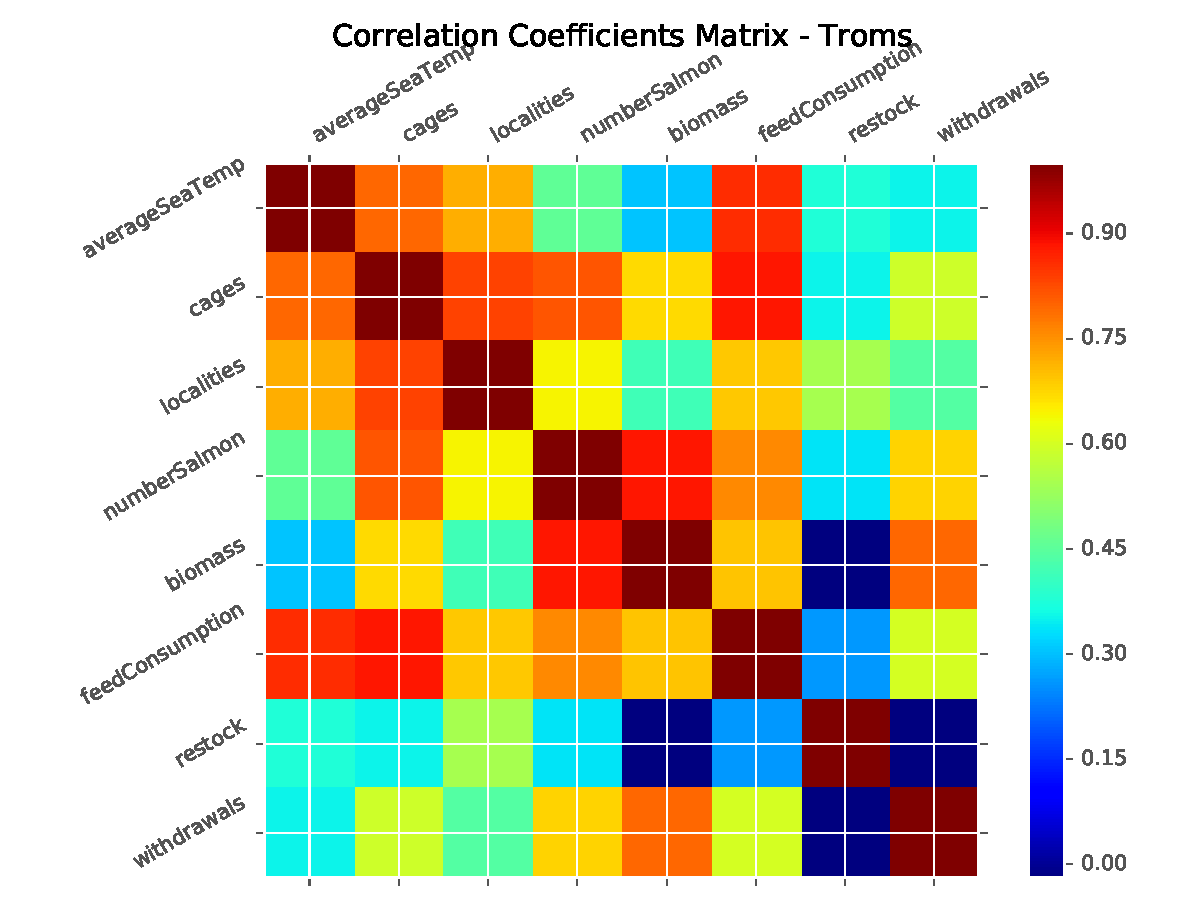
\includegraphics[trim={0 0 0 0},clip,width=1\textwidth]{Files/Troms_Total_Matrix.pdf}
    \caption[Correlation matrix between parameter of Troms dataset.]{Correlation matrix between all the parameters of the dataset about Troms}
    \label{fig: Troms_parametersComparison}
\end{figure}
\end{minipage}}
\makebox[1\textwidth][c]{
\begin{minipage}[t]{0.6\textwidth}
\begin{figure}[H]
    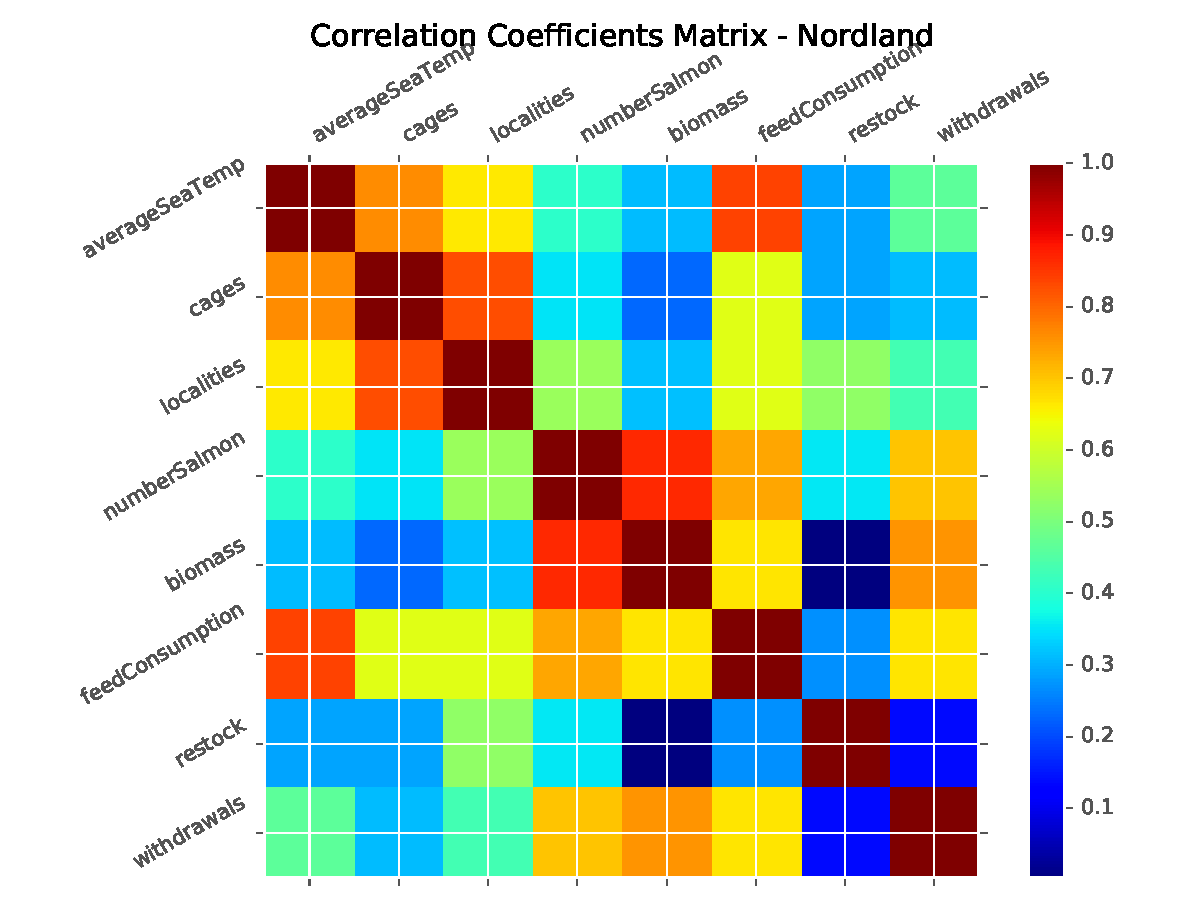
\includegraphics[trim={0 0 0 0},clip,width=1\textwidth]{Files/Nordland_Total_Matrix.pdf}
    \caption[Correlation matrix between parameter of Nordland dataset.]{Correlation matrix between all the parameters of the dataset about Nordland}
    \label{fig: Nordland_parametersComparison}
\end{figure}
\end{minipage} \hfill
\begin{minipage}[t]{0.6\textwidth}
\begin{figure}[H]
	\centering
    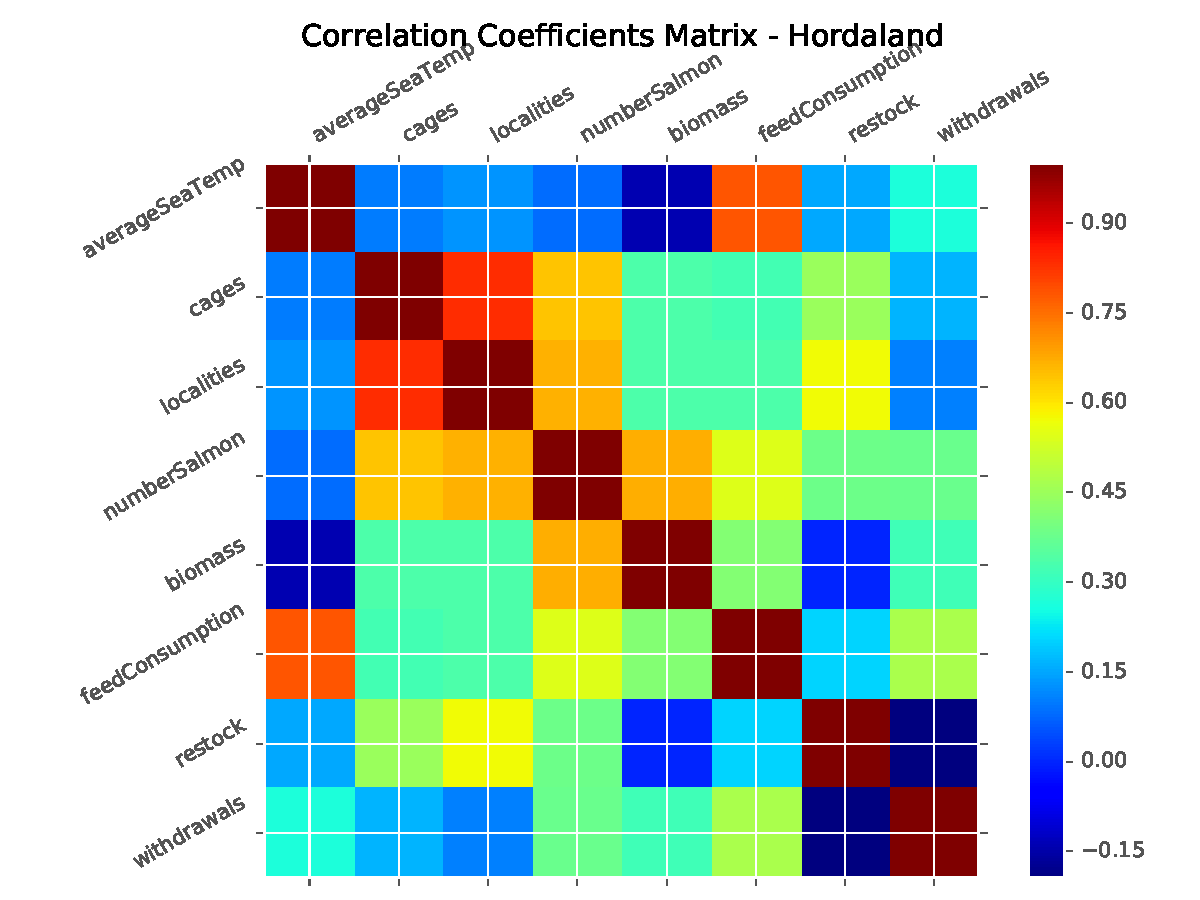
\includegraphics[trim={0 0 0 0},clip,width=1\textwidth]{Files/Hordaland_Total_Matrix.pdf}
    \caption[Correlation matrix between parameter of Hordaland dataset.]{Correlation matrix between all the parameters of the dataset about Hordaland}
    \label{fig: Hordaland_parametersComparison}
\end{figure}
\end{minipage}}


\section{Limitations of the study}
\vspace{-5mm}
This study has a number of limitations, mainly due to:
\vspace{-5mm}
\begin{itemize}
 \setlength{\itemsep}{-5pt}
  \item Hard to get access to salmon farming knowledge.
  \item Relatively short time available for this work since data access takes time.
\end{itemize}

As Senior Editor Amanda Hindle wrote, "No one expects science to be perfect the first time and while your peers can be highly critical, no one’s work is beyond limitations. Our knowledge base is built on uncovering each piece of the puzzle, one at a time, and limitations show us where new efforts need to be made. So much like peer review, don’t think of limitations as being inherently bad, but more an opportunity for a new challenge. In the end, your limitation may be someone else’s inspiration." \cite{limitations}

During this work I got more and more knowledge and experience mainly about the fields (Data Science procedures and Salmon farming in Norway), and it allowed to get anyway some positive and useful results that provide an answer to most of the initial objectives of this thesis. \\
  
